\section{NISAR: the 2026 Venezuela and Panama earthquakes}
\label{sec:nisar}

\subsection{Data}
We use NISAR's L-band PR products in the 40\,+\,5\,MHz mode, HH polarization.
\begin{itemize}
  \item \textbf{Venezuela}, four 12-day pairs spanning the 24 June 2026 events on the San Sebasti\'an fault:
        ascending tracks 61 (18--30 June) and 162 (13--25 June), and descending tracks 54 (17--29 June) and 126
        (22 June -- 4 July). Two frames per track.
  \item \textbf{Panama}, descending track 141, 27 September -- 9 October 2026, frames 84 and 85, spanning the
        9 October $M_w$\,7.7 earthquake.
\end{itemize}
Each pair is the first date's PR GSLC and the second date's RSLC geocoded onto its grids
(Appendix~\ref{app:registration}). The main band is multilooked to 50\,m, filtered (adaptive Goldstein
\citep{goldstein1998radar}) and unwrapped with SNAPHU, with a cut along the mapped rupture where the rupture would
otherwise be crossed (Venezuela's airport segment, all of D141). D141's south block is tied to the north at 34
cycles, one more than our range offsets gave it, by the side band (Section~\ref{sec:sbtie}). Every estimator of Section~\ref{sec:synthetic} runs on the cells, main-band unwrapping, fault-zone exclusion
and filter that made our screens. The \texttt{ours} arm reproduces the saved production screens to $4\times10^{-6}$\,rad on every track. The PR GUNW
of the same pair, made by ISCE3's \texttt{main\_diff\_ms\_band} with \texttt{unwrap\_correction: True}, is binned onto
the same cells, with its frames levelled on their overlap.

There is no truth here. The leak is measured as in the earlier comparisons: the slope of the screen's 15\,km
high-pass on that of the non-dispersive phase ($\phiA$ minus our screen), within 10\,km of the trace. That uses our
own screen as the reference for what is deformation. A second statistic avoids this: each screen's difference from
ours near the fault and far from it, and its step across the trace.

\subsection{Results}
\paragraph{Panama D141.} The rupture runs into the Gulf of Montijo at its west end and out of the swath at its east,
so the main band was unwrapped with a cut along the trace, and the block south of it was tied at 34 cycles
(Section~\ref{sec:sbtie}). Across the
trace, the non-dispersive phase steps by 197\,rad between 2--4\,km north and south, 3.8\,m of LOS. The double
difference therefore has to step by $0.044\times197 = 8.7$\,rad, 1.38 cycles, across a gap that no data bridge.
Every reformulated arm puts the south block one cycle of $\Delta$ off: within 10\,km of the trace their screens differ
from ours by up to 72.9\,rad (69\,rad for the wrapped one), whichever unwrapper is used. That includes the GUNW recipe on our cells, with or
without the fault-zone exclusion (Table~\ref{tab:nisar}, Fig.~\ref{fig:d141}). The two-band arms are off by several
cycles of the side band. Their leaks are positive (+0.12 to +0.16 reformulated, +1.2 to +1.5 two-band) because the
block's offset correlates with the step. Ours leaks $+0.001$ and steps $-8$\,mm across the trace. On the offsets' tie
it leaked $-0.005$ and stepped 17\,mm: the filter's mixing of a wrong tie (Section~\ref{sec:sbtie}).

The GUNW product itself is not one of these arms. Its main band was unwrapped without a cut and is 32 cycles off
across the rupture, because SNAPHU went around its end. Its double difference was unwrapped on the GUNW's own grid,
across the decorrelated fault zone, and the correction passes then ran on both. What results is the copy described in
Section~\ref{sec:intro}: a leak of $-0.104$ ($r=-0.81$), a 433\,mm step across the trace, and a difference from ours of
294\,mm rms within 10\,km. Most of it is the main band's integers. Averaged onto our cells, the product's unwrapped
phase is 25 cycles below ours on the south block and 3--9 above it within 30\,km north of the trace (ours is tied by
the side band). With that main band, even the reordered estimate leaks $-0.061$ ($r=-0.70$), and the GUNW recipe
$-0.056$. The reordering does not protect a screen from a wrong main band, at 3.21\,rad per cycle; on D141 the
remedy is the cut and the tie.

\paragraph{Venezuela.} The four tracks see a rupture that runs along the coast. North of the trace is sea for much
of its length, and the airport's cut-off block is left out of the estimate, so no cross-fault integer has to be
recovered. There the forms agree, as on the benign synthetics.
\begin{itemize}
  \item The reformulated estimate with our unwrapper equals ours on every track. With SNAPHU it differs only in local
        patches (on A061, up to 31\,rad within 10\,km of the trace). Taken as wrapped, it fails on D126, where $\Delta$
        spans more than a cycle.
  \item The two-band forms fail on every track: the side band's own unwrapping is off by cycles over much of the scene.
  \item The correction passes leak on every track (Fig.~\ref{fig:nisar}b). The GUNW recipe on our cells moves
        main-band cycles at 0.03--0.24\% of the cells and leaks 0.009--0.019 more than ours with the exclusion, and
        0.018--0.048 more without it.
\end{itemize}
Ours is not at zero: $+0.009$ on A061, $-0.036$ on D126, $-0.003$ on A162 and $+0.037$ on D054. Every non-failing arm
shares that value on its track, so it is the metric's floor there, not leakage. On D126 the rupture runs along a
coastline, and the 15\,km high-pass of a field that ends at the coast correlates with that of the near-fault
deformation. D054 carries real ionospheric waves 15--30\,km apart, which its GUNW screen shows too.

The products leak more: $-0.083$ ($r=-0.72$) on A061, $-0.123$ ($-0.82$) on D126, $-0.045$ ($-0.62$) on A162 and
$-0.021$ ($-0.19$) on D054. Beyond ours, that is 0.042--0.092. Two tests narrow down where it comes from.
\begin{itemize}
  \item Unlike D141's, these products' main band agrees with ours: the two differ by a whole cycle at 0.14\% of the
        cells or fewer, and at 0.3\% or fewer within 10\,km of the trace. With the products' main band, our estimate
        is unchanged and the recipe's leak moves by at most 0.004.
  \item Widening our side-band cells in range to the products' footprint (the side band multilooked over 325\,m of
        slant range against the main band's 40\,m; a $[0.365, 1, 0.365]$ kernel matches the second moment) changes
        every arm's leak on these tracks by at most 0.004.
\end{itemize}
The recipe on our cells thus accounts for 25--52\% of the products' leak beyond ours, and neither the main band's
integers nor the footprint mismatch accounts for the rest. That rest lies in steps our matched cells do not
reproduce: the products' own grid, their double difference unwrapped and bridged there, and their frame-by-frame
processing. We leave its attribution open.

\begin{table}[t]
\centering
\caption{The estimators on NISAR data, on identical cells: leak (slope and correlation of the screen's 15\,km
high-pass on the non-dispersive phase's, within 10\,km of the trace), the screen's step from 2--4\,km south to
2--4\,km north, and its difference from ours (both less their median beyond 20\,km), within 10\,km and beyond
20\,km. All in mm of LOS.}
\label{tab:nisar}
\scriptsize
\setlength{\tabcolsep}{4pt}
\begin{tabular}{llrrrrr}
\toprule
scene & estimator & leak & $r$ & step & \multicolumn{2}{c}{difference from ours} \\
 & & & & (mm) & $<$10\,km & $>$20\,km (mm) \\
\midrule
D141 & reordered (ours) & 0.001 & 0.32 & -7.8 & 0.0 & 0.0 \\
 & reformulated, same unwrapper & 0.136 & 0.72 & -682.8 & 931.7 & 136.3 \\
 & reformulated (SNAPHU) & 0.163 & 0.77 & -834.6 & 925.4 & 136.5 \\
 & ISCE3 recipe, no exclusion & 0.131 & 0.74 & -672.7 & 904.9 & 136.4 \\
 & two-band (SNAPHU) & 1.540 & 0.81 & -7417.3 & 7421.1 & 1079.4 \\
 & PR GUNW & -0.104 & -0.81 & 433.0 & 294.1 & 38.6 \\
\midrule
A061 & reordered (ours) & 0.009 & 0.42 & 22.3 & 0.0 & 0.0 \\
 & reformulated, same unwrapper & 0.009 & 0.42 & 22.3 & 0.0 & 0.0 \\
 & reformulated (SNAPHU) & 0.013 & 0.02 & 13.0 & 73.0 & 0.2 \\
 & ISCE3 recipe, no exclusion & -0.039 & -0.59 & 24.9 & 9.4 & 0.1 \\
 & two-band (SNAPHU) & 0.844 & 0.53 & -3.0 & 278.7 & 11.8 \\
 & PR GUNW & -0.083 & -0.72 & 21.4 & 18.6 & 7.3 \\
\midrule
D126 & reordered (ours) & -0.036 & -0.47 & 108.8 & 0.0 & 0.0 \\
 & reformulated, same unwrapper & -0.036 & -0.47 & 108.8 & 0.0 & 0.0 \\
 & reformulated (SNAPHU) & -0.036 & -0.47 & 108.8 & 0.0 & 0.2 \\
 & ISCE3 recipe, no exclusion & -0.057 & -0.65 & 99.3 & 5.4 & 0.8 \\
 & two-band (SNAPHU) & 0.069 & 0.51 & 109.0 & 12.5 & 278.1 \\
 & PR GUNW & -0.123 & -0.82 & 64.2 & 18.8 & 10.2 \\
\midrule
A162 & reordered (ours) & -0.003 & -0.11 & 15.6 & 0.0 & 0.0 \\
 & reformulated, same unwrapper & -0.003 & -0.11 & 15.6 & 0.0 & 0.0 \\
 & reformulated (SNAPHU) & -0.003 & -0.09 & 15.5 & 0.2 & 0.3 \\
 & ISCE3 recipe, no exclusion & -0.025 & -0.45 & 17.6 & 5.0 & 0.4 \\
 & two-band (SNAPHU) & 1.515 & 0.55 & 10.8 & 310.8 & 560.5 \\
 & PR GUNW & -0.045 & -0.62 & 18.1 & 12.2 & 7.6 \\
\midrule
D054 & reordered (ours) & 0.037 & 0.39 & 1.4 & 0.0 & 0.0 \\
 & reformulated, same unwrapper & 0.037 & 0.39 & 1.4 & 0.0 & 0.0 \\
 & reformulated (SNAPHU) & 0.037 & 0.39 & 1.4 & 0.0 & 0.0 \\
 & ISCE3 recipe, no exclusion & 0.019 & 0.19 & -2.5 & 5.3 & 0.5 \\
 & two-band (SNAPHU) & 0.916 & 0.51 & -0.7 & 250.3 & 37.8 \\
 & PR GUNW & -0.021 & -0.19 & -16.8 & 11.1 & 8.2 \\
\bottomrule
\end{tabular}

\end{table}

\begin{figure}[t]
\centering
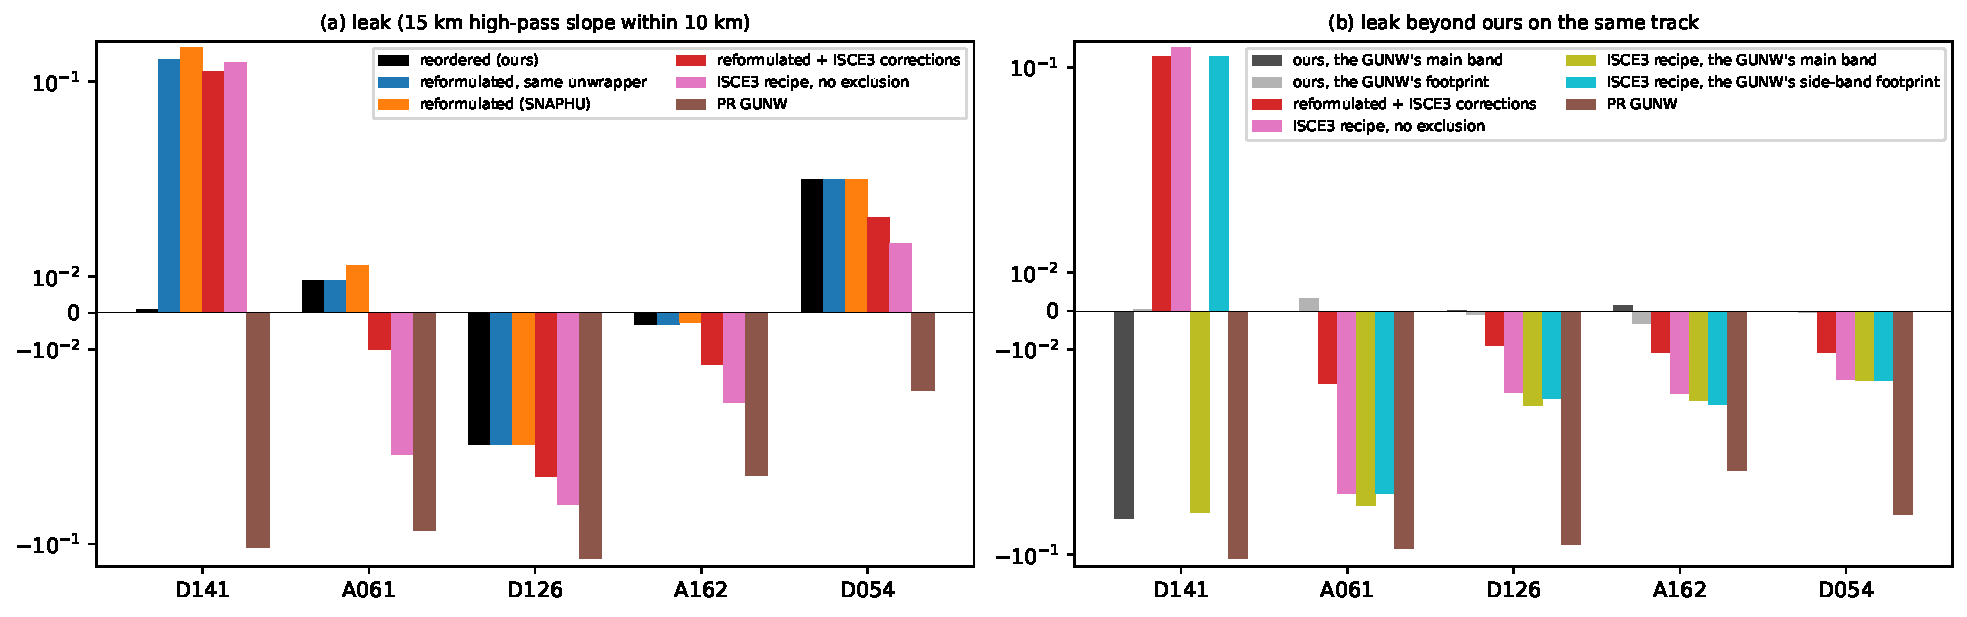
\includegraphics[width=\textwidth]{figures/fig_nisar}
\caption{The leak on the five NISAR tracks. (a) Each estimator on our cells, and the PR GUNW. (b) The leak beyond
ours on the same track, which removes each track's floor (the value every non-failing arm shares). It shows the GUNW
recipe on our cells, the same with the product's own main band or the product's side-band footprint, and the product.
Symmetric log scale.}
\label{fig:nisar}
\end{figure}

\begin{figure}[t]
\centering
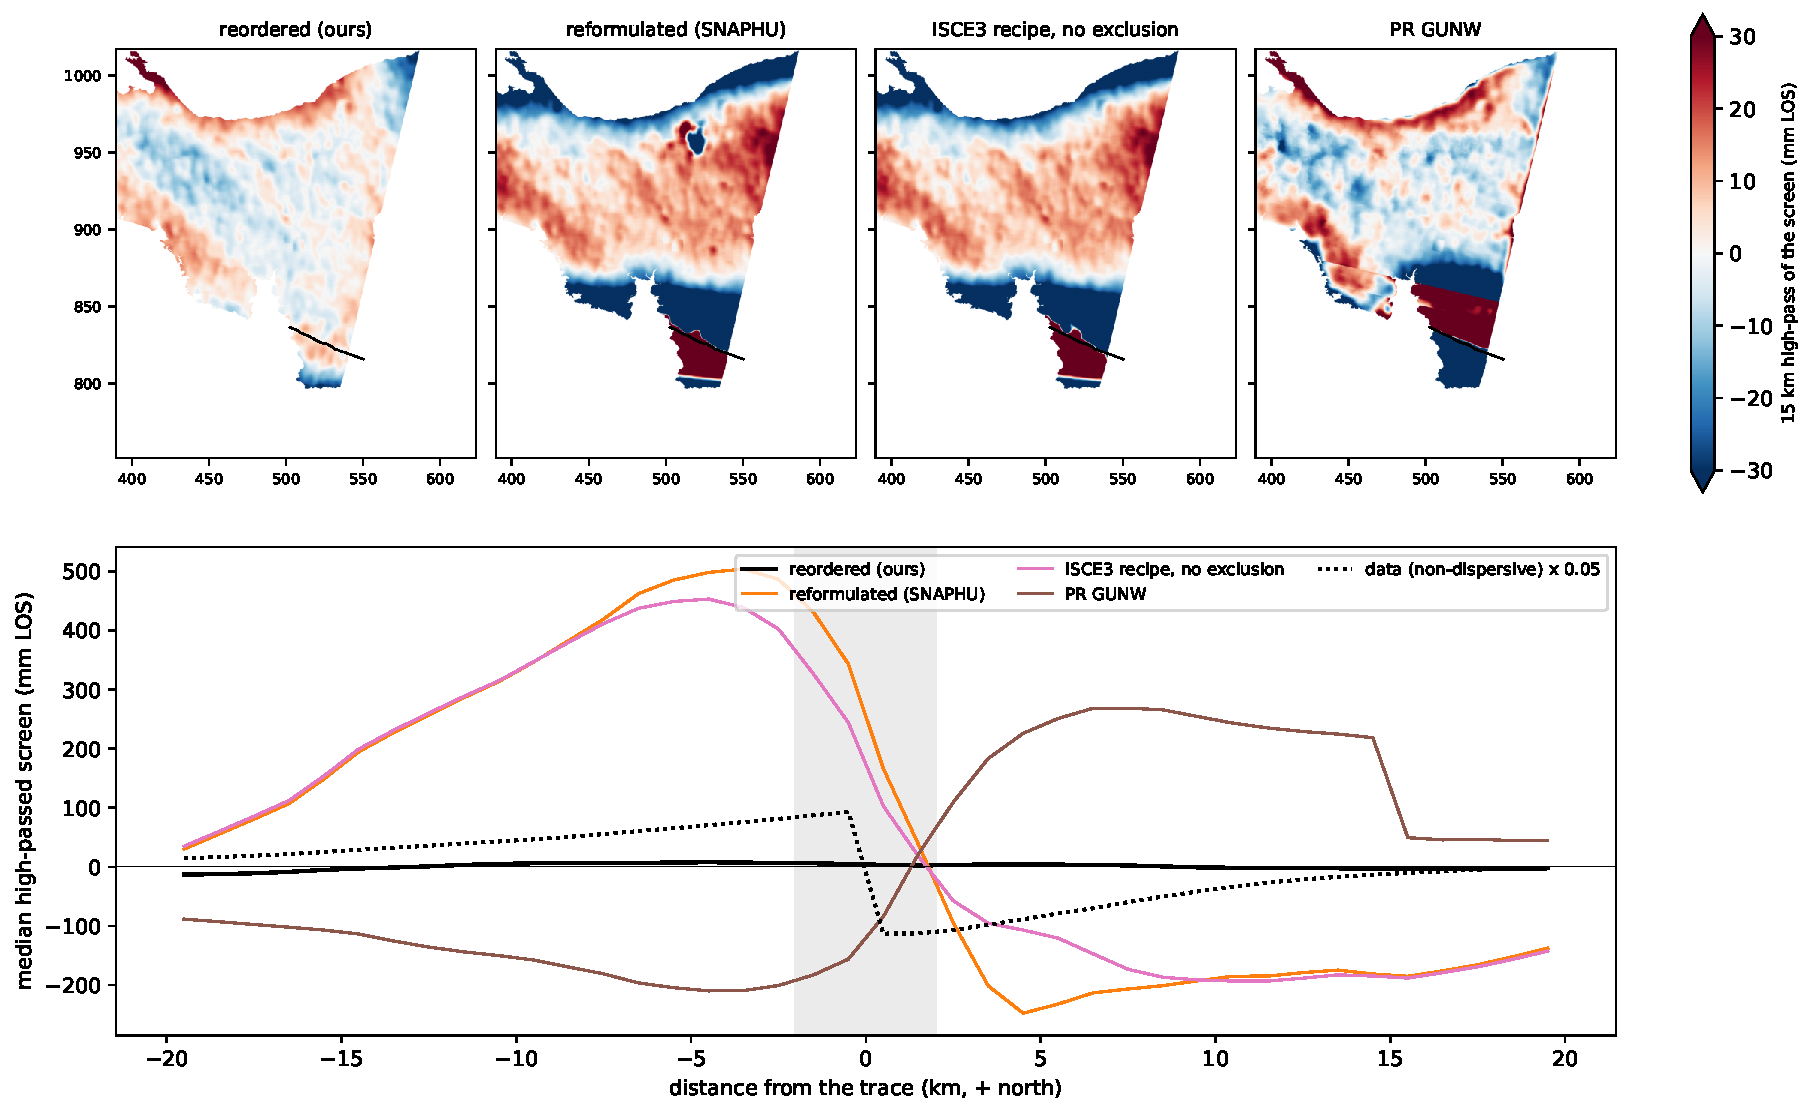
\includegraphics[width=\textwidth]{figures/fig_d141}
\caption{Panama D141. The 15\,km high-pass of four screens on identical cells: ours, the reformulated estimate with
SNAPHU, the GUNW recipe on our cells (no exclusion), and the PR GUNW product. Below: their median across the
trace, with the data's high-pass ($\times0.05$) for reference.}
\label{fig:d141}
\end{figure}
